\section{Development process and implementation}
\label{chap:development_process}

This chapter details the steps used during the development of the program. Features of the program were added iteratively, beginning with simply getting the LEDs to light up and then evolving to more sophisticated funcionality. The first iteration of the code simply turned on the LEDs. After this, an opening sequence was added to the program, the details of which and why it was added is explained more in section \ref{subsec:dev_pros_opening_seq}. Afterwards, a polling technique was used to test the buttons on the game pad. With the correct flags set a number will be written to a specific location in memory which indicates what buttons are being pressed. This number is then shifted eight places to the left to comply with the way LEDs are lightened up.

The next step was to make interrupts work. A main function was constructed to set the correct flags. When these are set the device goes to sleep and waits for an interrupt. A main focus was to abort the interrupts as quickly as possible. More on this in section \ref{subsec:dev_pros_interrupts}.

\subsection{Pre-assignment setup}
\label{subsec:pre-assingment_setup}

The assignment involves a lot of GPIO usage, and therefore some values are used over and over. The register design is set up so that three registers are storing GPIO constants and one register is used for simulating a wait for the opening sequence. They each have an alias to be easier to access. GPIO\_PA\_BASE was renamed gpio\_o and GPIO\_PC\_BASE was renamed to gpio\_i, GPIO\_BASE was renamed gpio. The remaining registers from r0 to r7 is used for variable content. See table \ref{tab:register_design} in appendix A on page \pageref{tab:register_design} for an overview of the registers.

\subsection{Setting up the LEDs}
\label{subsec:dev_pros_setup_led}

The LEDs are connected to the EFM32 through the GPIO. To enable the GPIO, the clock needs to be enabled for the GPIO controller. The CMU is responsible for the clock and is fortunately very easy to use. Register CMU\_HFPERCLKEN0 is a 32 bits register with each bit correponding to a specific IO controller. The GPIO controller is on the 13th bit, and after that bit has been set to 1, the GPIO is ready for use.

\begin{figure}[h!]
\begin{code}
// C-equivalent:
// *CMU_HFPERCLKEN0 |= (1 << 13)
ldr r1, =CMU_BASE
ldr r2, [r1, #CMU_HFPERCLKEN0]
mov r3, #1
lsl r3, r3, #CMU_HFPERCLKEN0_GPIO
orr r2, r2, r3
str r2, [r1, #CMU_HFPERCLKEN0]
\end{code}
\caption{Enable CMU for GPIO}
\label{code:enable_cmu_gpio}
\end{figure}

The GPIO has multiple connections. The game pad is connected so that button presses are registered on the C connection and which lights should be on is read from the A connection. Following this, the drive strength of the light is set on the A connection. This can take one of four values, each corresponding to a different Ampère setting. Table \ref{tab:drive_strength} in appendix A on page \pageref{tab:drive_strength} shows the different settings for drive strength. To save power, the strength should be set as low as possible, but for this assignment the power consumption of the LEDs are ignored and therefore the drive strength is set to high.

\begin{figure}[h!]
\begin{code}
mov r2, #0x2
str r2, [gpio_o, #GPIO_CTRL]
\end{code}
\caption{Set drive strength for GPIO OUTPUT}
\label{code:set_drive_gpio_o}
\end{figure}

The pins on the game pad is connected to the top 8 pins on the EFM32GG-DK3750 development kit. The constant 0x55555555 is written to the GPIO\_PA\_MODEH register, this so the pins is set to output.

\begin{figure}[h!]
\begin{code}
mov r2, #0x55555555
str r2, [gpio_o, #GPIO_MODEH]
\end{code}
\caption{Set pins to output}
\label{code:set_drive_gpio_o}
\end{figure}

\subsection{Setting up buttons on the gamepad}
\label{subsec:dev_pros_button_setup}
The program itself has a boot sequence after the LEDs are set up, the details of this can be read in section \ref{subsec:dev_pros_opening_seq}.

The next operation sets the gamepad buttons up for input. All of the setup has been done by the setup of the LEDs, so there is no need for that. To enable the pins for input, writing 0x33333333 to GPIO\_PC\_MODEL is needed. To enable internal pull-up 0xff is written to GPIO\_PC\_DOUT. After this the buttons pressed in can be read from bits 0-7 of GPIO\_PC\_DIN and the LEDs will light up by writing to bits 8-15 of GPIO\_PA\_DOUT.

\begin{figure}[h!]
\begin{code}
mov r2, #0x33333333
str r2, [gpio_i, #GPIO_MODEL]
mov r2, #0xff
str r2, [gpio_i, #GPIO_DOUT]
\end{code}
\caption{Enable buttons for gamepad}
\label{code:set_drive_gpio_o}
\end{figure}

\subsection{Opening sequence}
\label{subsec:dev_pros_opening_seq}

The program provides an opening sequence testing the LEDs for the convenience of the user. This subsection outlines the implementation of the opening sequence and implications it provides. A slow motion YouTube video of the opening sequence is available at: \url{http://youtu.be/PJpPFoC9Jtg}. The video is four times slower than real life.

To make the LEDs light up one by one with a small timeframe in between, a casual wait loop was created. This loop simulates a wait by branching out to a loop and subtracting a small value from a large number. It then checks if the result is zero, if not it repeats the process. With a large enough number this will take a small fraction of a second which is exactly what is needed. A special register cw is reseved for this purpose. See figure \ref{code:casual_wait}.

To light up the LEDs, different values are written to GPIO\_PA\_DOUT. After a value is written, one iteration of the casual wait is performed. To make the lights light up and down in a row, a simple bitshift is done to the right and the left respectively. The end effect is a bigger one. It needs all lights to be shut off at the start and has the following formula.

$$ \texttt{out = ((out \& 0xf000) << 1 | (out \& 0x0f00) >> 1) \& 0xff00} $$

Out in the formula is in our case GPIO\_PA\_DOUT.


\begin{figure}[h!]
\begin{code}
casual_wait:
    mov cw, #0x000a0000
cwait_loop:
    subs cw, #1
    bne cwait_loop
    bx lr
\end{code}
\caption{Casual wait – simulating a wait for the LED test}
\label{code:casual_wait}
\end{figure}

\subsection{Reading button status using polling}
\label{subsec:polling}

The most naïve way to use button input is by reading the input continuously and writing the input data to the LEDs.
As seen in Figure \ref{code:polling}, the main loop first loads the data from GPIO\_PC\_DIN.
It is then shifted 8 bits to the left and written to GPIO\_PA\_DOUT.
When the operation is complete, the program branches back to the main\_loop label and thus continues forever.
The results section will present the differences in power consumption between this method and using interrupt triggered input checking.

\begin{figure}[h!]
\begin{code}
main_loop:
    ldr r2, [gpio_i, #GPIO_DIN]
    lsl r2, r2, #8
    str r2, [gpio_o, #GPIO_DOUT]
    b main_loop
\end{code}
\caption{Naïve continuous checking of input status}
\label{code:polling}
\end{figure}

\subsection{Programming with interrupts}
\label{subsec:dev_pros_interrupts}

Interrupt support is implemented by first setting up the interrupt handlers.
Then, we activate the pins corresponding to the buttons by writing 0x22222222 to GPIO\_EXTIPSELL.
We further activate the External Interrupt Rising Edge Trigger, and the External Interrupt Falling Edge Trigger by writing 0xff to the GPIO\_EXTIRISE and GPIO\_EXTIFALL registers respectively.
Interrupt generation is enabled by writing 0xff to GPIO\_IEN.
To finally implement handling of interrupts, we set the two bits in ISER0 corresponding to our handler to 1. They are bit 1 and 11 in the register, resulting in the hexadecimal representation 0x802.
The code required for setting up interrupts can be seen in figure \ref{code:interrupt_setup}.

\begin{figure}[h!]
\begin{code}
mov r2, #0x22222222
str r2, [gpio, #GPIO_EXTIPSELL]
mov r2, #0xff
str r2, [gpio, #GPIO_EXTIFALL]
str r2, [gpio, #GPIO_EXTIRISE]
str r2, [gpio, #GPIO_IEN]
ldr r2, =0x802
ldr r3, =ISER0
str r2, [r3, #0]
\end{code}
\caption{Code for enabling interrupts generation and handling}
\label{code:interrupt_setup}
\end{figure}


The first thing that the GPIO handler takes care of is to clear the interrupt. If this is not done, the handler will be called again as if the buttons are still being pressed.

\subsection{Deep sleep}
\label{subsec:dev_pros_deep_sleep}

When interrupt handlers are implemented, the CPU is able to sleep when there is no processing to be done.
Deep sleep is a mode with a power consumption of only 1.1 \si{\micro\ampere}.
This is achieved by disabling the high-frequency oscillator, and instead using a lower-frequency one.
Many of the more power-consuming peripherals are also disabled in this mode.

To activate deep sleep mode we must set bit number 2 of the System Control Register to 1, as seen in figure \ref{code:deep_sleep}

\begin{figure}[h!]
\begin{code}
ldr r2, =0x4
ldr r3, =SCR
str r2, [r3, #0]
\end{code}
\caption{Enabling deep sleep}
\label{code:deep_sleep}
\end{figure}

Since we are working with interrupts, we also want the CPU to go back to sleep when an interrupt has been handled.
The System Control Register has a flag for this functionality as well, in bit number 1.
We therefore write 0x6 to the SCR to enable both deep sleep and sleep on exit (see figure \ref{code:deep_sleep_on_exit}).

\begin{figure}[h!]
\begin{code}
ldr r2, =0x6
ldr r3, =SCR
str r2, [r3, #0]
\end{code}
\caption{Enabling both deep sleep and sleep on exit}
\label{code:deep_sleep_on_exit}
\end{figure}

\subsection{Energy Mode 4}
\label{subsec:em4}

There is an energy mode 4 that the EFM32 supports. This mode uses next to no power and disables most of the controllers, but this doesn't come for free. EM4 disables so many key components that it's impossible to wake it up again via the interrupts used in energy mode 2.

One sollution would be to have an extra hardware expansion from each button directly to the interrupt handler that wakes the microcontroller up from EM4. This is not so practical for every application and even in this instance is more than a slight impracticality.

Even if the interrupt was easier to handle EM4 would not be desired for this use. The buttons are most likely going to be pressed multiple times within a small time interval. The graph on Figure \ref{fig:em4} taken from EFM32 Energy Optimization Application Note \cite{efm32-energy-op} shows that EM4 takes a longer time to use less power. This means that it's ideal for when the microcontroller should stay idle for a long time. In this case it would use less power to be on EM2 than on EM4.

\begin{figure}[h!]
    \begin{center}
    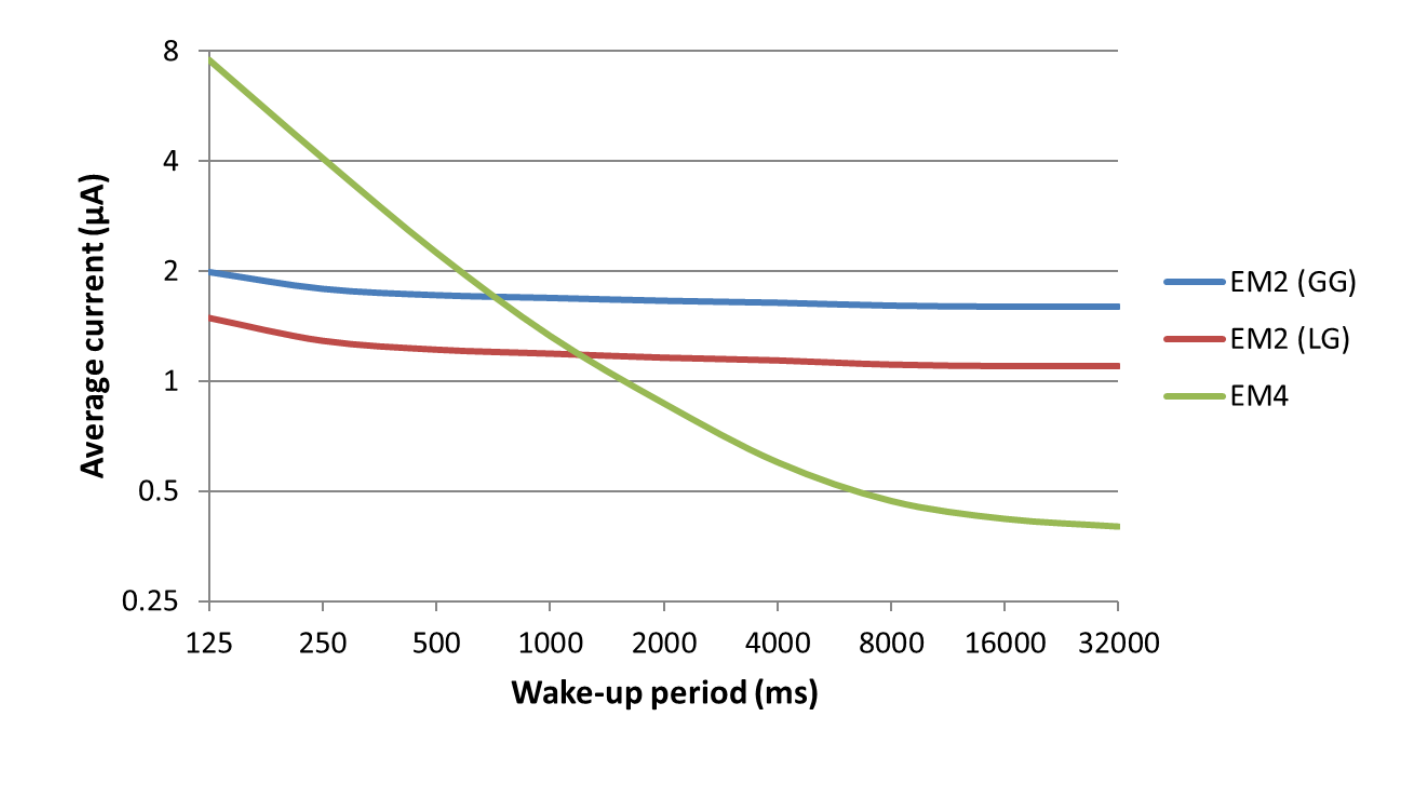
\includegraphics[width=0.8\textwidth]{assets/img/em4.png}
    \caption{The power usage for EM4 against EM2 on the Giant Gecko and Leopard Gecko}
    \label{fig:em4}
    \end{center}
\end{figure}
